% Добавлена опция usepdftitle=false, которая запрещает Beamer автоматически передавать верстку автора в метаданные PDF
\documentclass[aspectratio=169, xcolor={table}, usepdftitle=false]{beamer} % Формат 16:9

\usepackage{cmap} % Для корректного поиска и копирования кириллицы из PDF
\usepackage[T2A]{fontenc}
\usepackage[utf8]{inputenc}
\usepackage[russian]{babel}
\usepackage{PTSans} % Векторный шрифт без засечек
\usepackage{graphicx}
\usepackage{xspace}
\usepackage{psfrag}
\usepackage{hyperref}
\usepackage[normalem]{ulem}
\usepackage{amsmath} % Пакет для математических формул и текста в индексах

% Ручное и безопасное указание метаданных PDF без сложной верстки
\hypersetup{
  pdftitle={Создание интеллектуальных ассистентов для инженерных продуктов на примере узкоспециализированных предметных областей},
  pdfauthor={Михайлов Николай Кириллович}
}

\beamertemplatenavigationsymbolsempty
\setbeamertemplate{footline}[frame number]
\usecolortheme{seahorse}

% Цвет для заголовков таблиц из вашей презентации
\definecolor{tabgreen}{HTML}{92D050}

%%Исправляем греческие буквы в формулах
\DeclareSymbolFont{greek}{U}{eur}{m}{n}                                                        
\SetSymbolFont{greek}{bold}{U}{eur}{b}{n}                                                      
\DeclareSymbolFontAlphabet{\gr}{greek}                                                         
\DeclareMathSymbol{\alpha}{\mathord}{greek}{"0B}                                               
\DeclareMathSymbol{\beta}{\mathord}{greek}{"0C}                                                
\DeclareMathSymbol{\gamma}{\mathord}{greek}{"0D}                                               
\DeclareMathSymbol{\delta}{\mathord}{greek}{"0E}                                               
\DeclareMathSymbol{\epsilon}{\mathord}{greek}{"0F}                                             
\DeclareMathSymbol{\zeta}{\mathord}{greek}{"10}                                                
\DeclareMathSymbol{\eta}{\mathord}{greek}{"11}                                                 
\DeclareMathSymbol{\theta}{\mathord}{greek}{"12}                                               
\DeclareMathSymbol{\iota}{\mathord}{greek}{"13}                                                
\DeclareMathSymbol{\kappa}{\mathord}{greek}{"14}                                               
\DeclareMathSymbol{\lambda}{\mathord}{greek}{"15}                                              
\DeclareMathSymbol{\mu}{\mathord}{greek}{"16}                                                  
\DeclareMathSymbol{\nu}{\mathord}{greek}{"17}                                                  
\DeclareMathSymbol{\xi}{\mathord}{greek}{"18}                                                  
\DeclareMathSymbol{\pi}{\mathord}{greek}{"19}                                                  
\DeclareMathSymbol{\rho}{\mathord}{greek}{"1A}                                                 
\DeclareMathSymbol{\sigma}{\mathord}{greek}{"1B}                                               
\DeclareMathSymbol{\tau}{\mathord}{greek}{"1C}                                                 
\DeclareMathSymbol{\upsilon}{\mathord}{greek}{"1D}                                             
\DeclareMathSymbol{\phi}{\mathord}{greek}{"1E}                                                 
\DeclareMathSymbol{\chi}{\mathord}{greek}{"1F}                                                 
\DeclareMathSymbol{\psi}{\mathord}{greek}{"20}                                                 
\DeclareMathSymbol{\omega}{\mathord}{greek}{"21}                                               
\DeclareMathSymbol{\varepsilon}{\mathord}{greek}{"22}                                          
\DeclareMathSymbol{\vartheta}{\mathord}{greek}{"23}                                            
\DeclareMathSymbol{\varpi}{\mathord}{greek}{"24}                                               
\let\varrho\rho                                                                                
\let\varsigma\sigma                                                                            
\DeclareMathSymbol{\varphi}{\mathord}{greek}{"27}

% Настройка титульного листа
\title{Создание интеллектуальных ассистентов для инженерных продуктов на примере узкоспециализированных предметных областей}
\author{%
  \begin{tabular}{rl}
    Студент: & Михайлов Николай Кириллович, гр. 932302 \\[0.3cm]
    Научный руководитель: & канд. т. н. Пожидаев Михаил Сергеевич
  \end{tabular}
}
\date{} 

\begin{document}

% --- Слайд 1 ---
\begin{frame}
\maketitle
\end{frame}

% --- Слайд 2 ---
\begin{frame}
\frametitle{Объект и предмет исследования}
\textbf{Объект исследования:} алгоритмы извлечения и генерации информации с использованием больших языковых моделей (LLM) и технология дополненного поиска \\[0.5cm]
\textbf{Предмет исследования:} архитектурные методы и алгоритмические стратегии, определяющие точность и полноту извлечения знаний в RAG-системах
\end{frame}

% --- Слайд 3 ---
\begin{frame}
\frametitle{Цель исследования}
\Large
Создание RAG-системы, обеспечивающей высокую достоверность и минимизацию информационного шума при работе с документацией программных продуктов для узкоспециализированных предметных областей.
\end{frame}

% --- Слайд 4 (Схема 1) ---
\begin{frame}
\begin{center}
    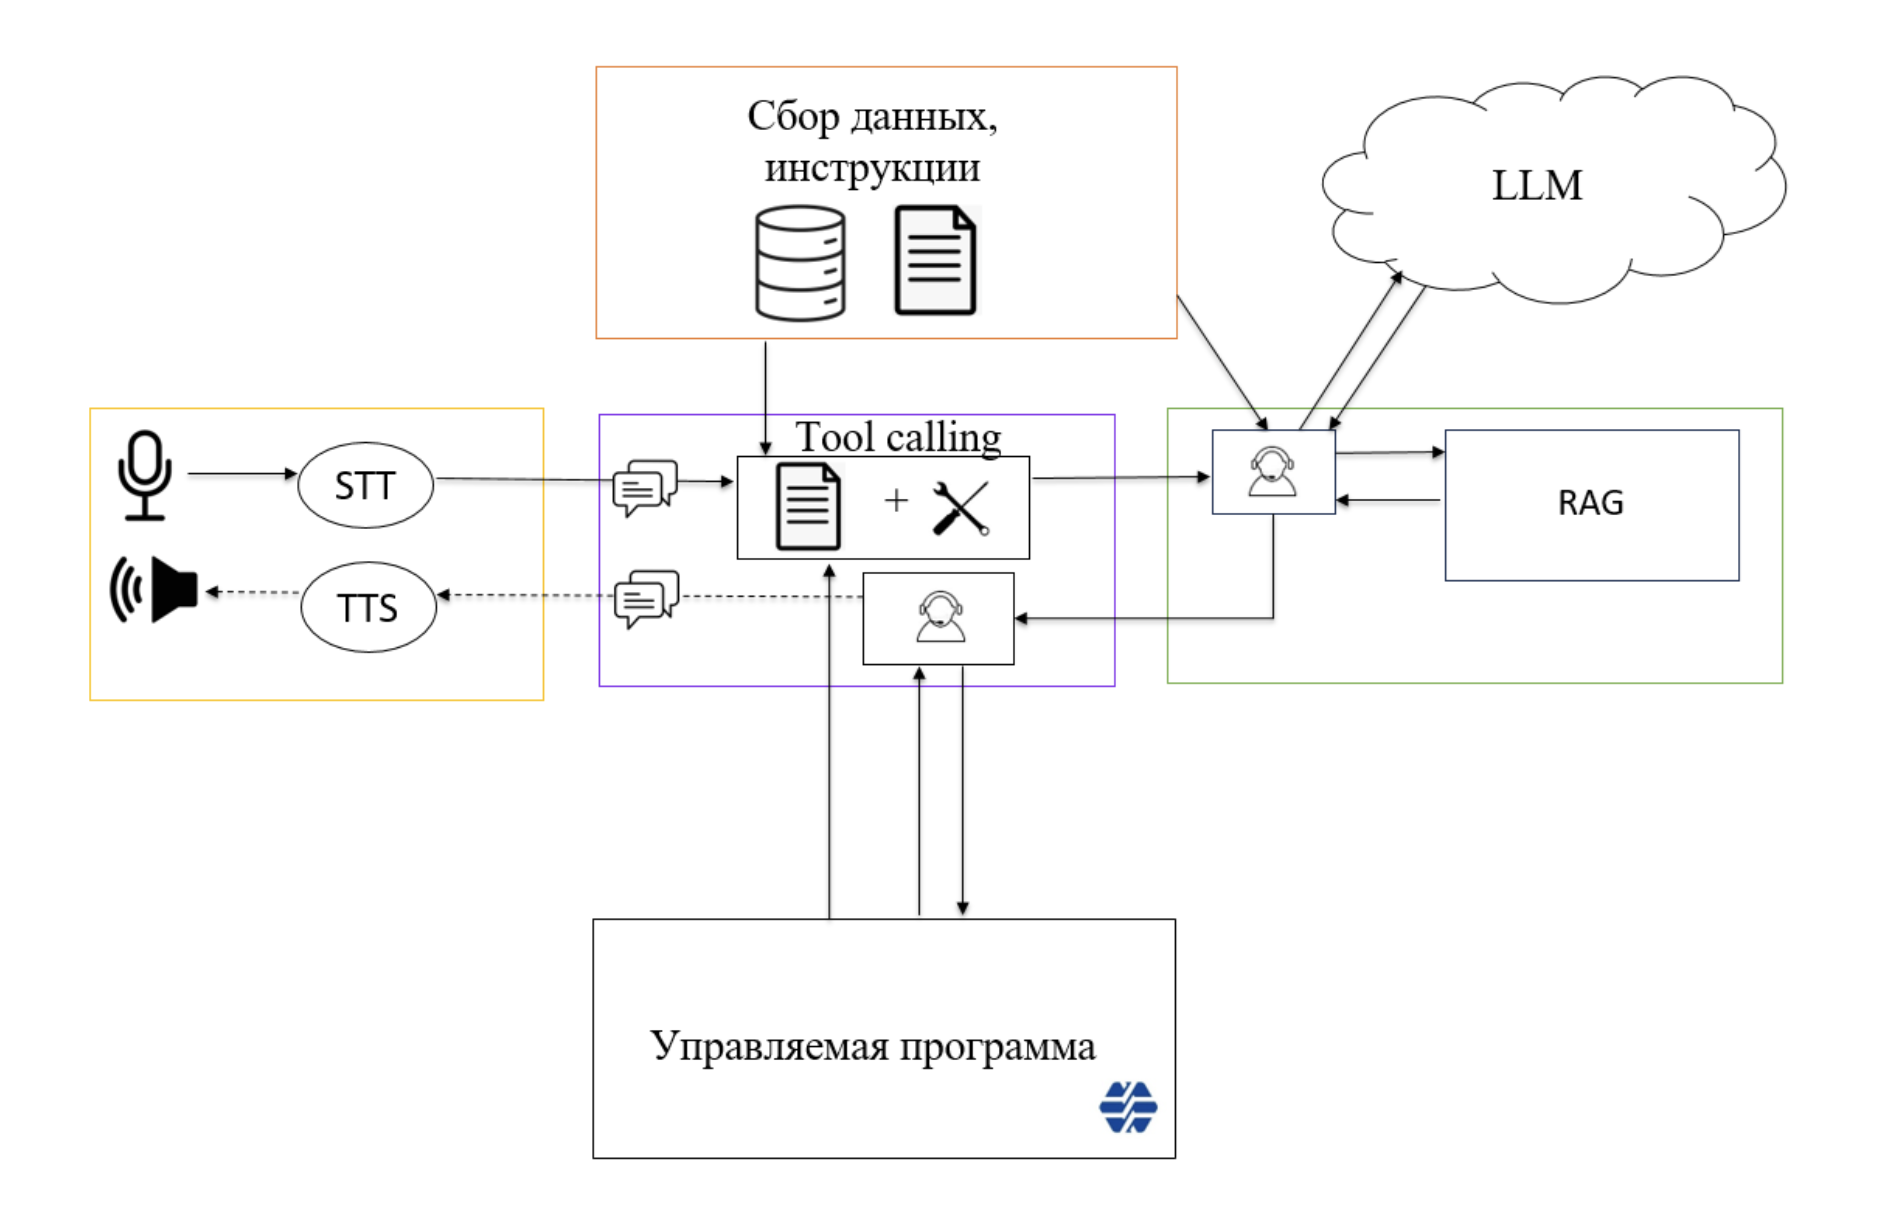
\includegraphics[width=\textwidth, height=0.95\textheight, keepaspectratio]{scheme1.jpeg}
\end{center}
\end{frame}

% --- Слайд 5 ---
\begin{frame}
\frametitle{Задачи}
\small
\begin{enumerate}
    \item Провести теоретический анализ существующих поколений архитектур RAG.
    \item Адаптировать и локализовать методику автоматизированной оценки RAGAS.
    \item Разработать стратегию специализированной предобработки данных, включающую иерархическую нарезку текста, для сохранения логической структуры инженерной документации.
    \item Реализовать модуль семантической оптимизации запросов.
    \item Спроектировать механизм глобального гибридного поиска.
    \item Провести сравнительный анализ эффективности различных LLM.
    \item Провести сравнительное тестирование современных эмбеддеров.
    \item Интегрировать механизмы заключительной обработки.
\end{enumerate}
\end{frame}

% --- Слайд 6 ---
\begin{frame}
\frametitle{Эволюция архитектурных подходов RAG}
\small
\begin{enumerate}
    \item \textbf{Naive RAG (базовый подход): прямой поиск и генерация}
    \begin{itemize}
        \item \underline{Суть процесса:} прямая передача найденных документов в LLM без предварительного отбора.
        \item \underline{Недостатки:} высокий уровень семантического шума, передача нерелевантного контекста, низкая точность в узкоспециализированных предметных областях.
    \end{itemize}
    \vspace{0.2cm}
    \item \textbf{Advanced RAG (продвинутый подход): введение предобработки запроса и обработки найденного контекста}
    \begin{itemize}
        \item \underline{Суть процесса:} оптимизация данных на этапах до поиска (предобработка) и после извлечения (реранжирование, фильтрация по порогам релевантности).
        \item \textbf{!!! Этот подход является основой данной курсовой работы}
    \end{itemize}
    \vspace{0.2cm}
    \item \textbf{Modular RAG (модульный подход): гибкая перестановка модулей и итеративный поиск}
    \begin{itemize}
        \item \underline{Суть процесса:} использование независимых функциональных блоков, динамической маршрутизации запросов и циклов самокоррекции (Self-RAG).
        \item \underline{Недостатки:} высокая сложность развертывания и отладки.
    \end{itemize}
\end{enumerate}
\end{frame}

% --- Слайд 7 ---
\begin{frame}
\frametitle{Автоматизированная оценка (RAGAS)}
\small
\textbf{Faithfulness (достоверность):} контроль отсутствия галлюцинаций. Сгенерированный системой ответ разбивается на атомарные утверждения, и каждое из них проверяется на строгое соответствие найденному контексту. 
\vspace{0.3cm}

\textbf{Context Precision (точность контекста):} оценка релевантности поиска. Каждый извлеченный фрагмент текста проверяется на смысловое соответствие исходному запросу пользователя.
\vspace{0.3cm}

\textbf{Context Recall (полнота контекста):} проверка достаточности найденной информации. Факты из идеального (эталонного) ответа сопоставляются с извлеченным контекстом.
\vspace{0.3cm}

\textbf{Answer Accuracy (точность ответа):} итоговое соответствие эталону. Независимая языковая модель (LLM-судья) сопоставляет сгенерированный ответ с идеальным по строгим семантическим критериям (факты, цифры, даты) и выставляет усредненную оценку на основе двух независимых проверок.
\end{frame}

% --- Слайд 8 (Формулы) ---
\begin{frame}
\frametitle{Формулы рассчитываемых метрик}
\Large
\begin{enumerate}
    \setlength{\itemsep}{10pt}
    \item Faithfulness \hspace{2cm} $F = \frac{|S_{\text{supported}}|}{|S_{\text{total}}|}$
    
    \item Context Precision \hspace{1cm} $CP = \frac{|C_{\text{relevant}}|}{|C_{\text{total}}|}$
    
    \item Context Recall \hspace{1.7cm} $CR = \frac{|G_{\text{supported}}|}{|G_{\text{total}}|}$
    
    \item Answer Accuracy \hspace{1.3cm} $AA = \frac{\frac{Score_1}{4} + \frac{Score_2}{4}}{2}$
\end{enumerate}
\end{frame}

% --- Слайд 9 ---
\begin{frame}
\frametitle{Сохранение структуры документа}
\textbf{Проблема: утрата контекста при линейном разбиении}
\begin{itemize}
    \item При стандартном делении текста на фрагменты равной длины чанки отрываются от своих заголовков. В результате извлеченный фрагмент теряет смысловую связь с темой раздела, что приводит к неточным ответам модели на узкоспециализированных документах.
\end{itemize}
\vspace{0.5cm}

\textbf{Решение: структурное разбиение и иерархическое обогащение метаданными}
\begin{itemize}
    \item Документ сегментируется с учетом разметки. Каждый текстовый фрагмент снабжается метаданными, хранящими цепочку родительских заголовков. При поиске модель получает чанк вместе с его ``адресом'' в документе, что сохраняет полный контекст модели.
\end{itemize}
\end{frame}

% --- Слайд 10 ---
\begin{frame}
\frametitle{Семантическая оптимизация запросов}
\textbf{Query Expansion (расширение запроса):} генерация нескольких синонимичных вариантов исходного запроса с помощью большой языковой модели. Это позволяет учесть различия в терминологии (профессиональные термины, аббревиатуры, синонимы) и повышает вероятность нахождения нужных документов в базе данных.
\vspace{0.5cm}

\textbf{HyDE (гипотетический документ):} создание предварительного гипотетического ответа на запрос пользователя до обращения к базе данных. Поиск по вектору готового ответа семантически более точен, так как структура утвердительного предложения ближе к целевым документам в базе, чем структура вопросительного предложения.
\end{frame}

% --- Слайд 11 ---
\begin{frame}
\frametitle{Гибридный поиск}
\textbf{Dense Retrieval (векторный поиск по смыслу):} поиск документов на основе их семантического значения с использованием эмбеддингов.
\vspace{0.4cm}

\textbf{Sparse Retrieval (лексический поиск по ключевым словам):} поиск по точным текстовым совпадениям.
\vspace{0.4cm}

\textbf{Метод объединения (Reciprocal Rank Fusion / RRF):} алгоритм слияния результатов векторного и лексического поиска в единый сортированный список. RRF оценивает документы на основе их взаимного расположения (ранга) в обоих списках, что решает проблему несовместимости сырых математических оценок разных поисковых систем.
\end{frame}

% --- Слайд 12 (Схема 2) ---
\begin{frame}
\frametitle{Итоговая цепочка обработки запроса}
\begin{center}
    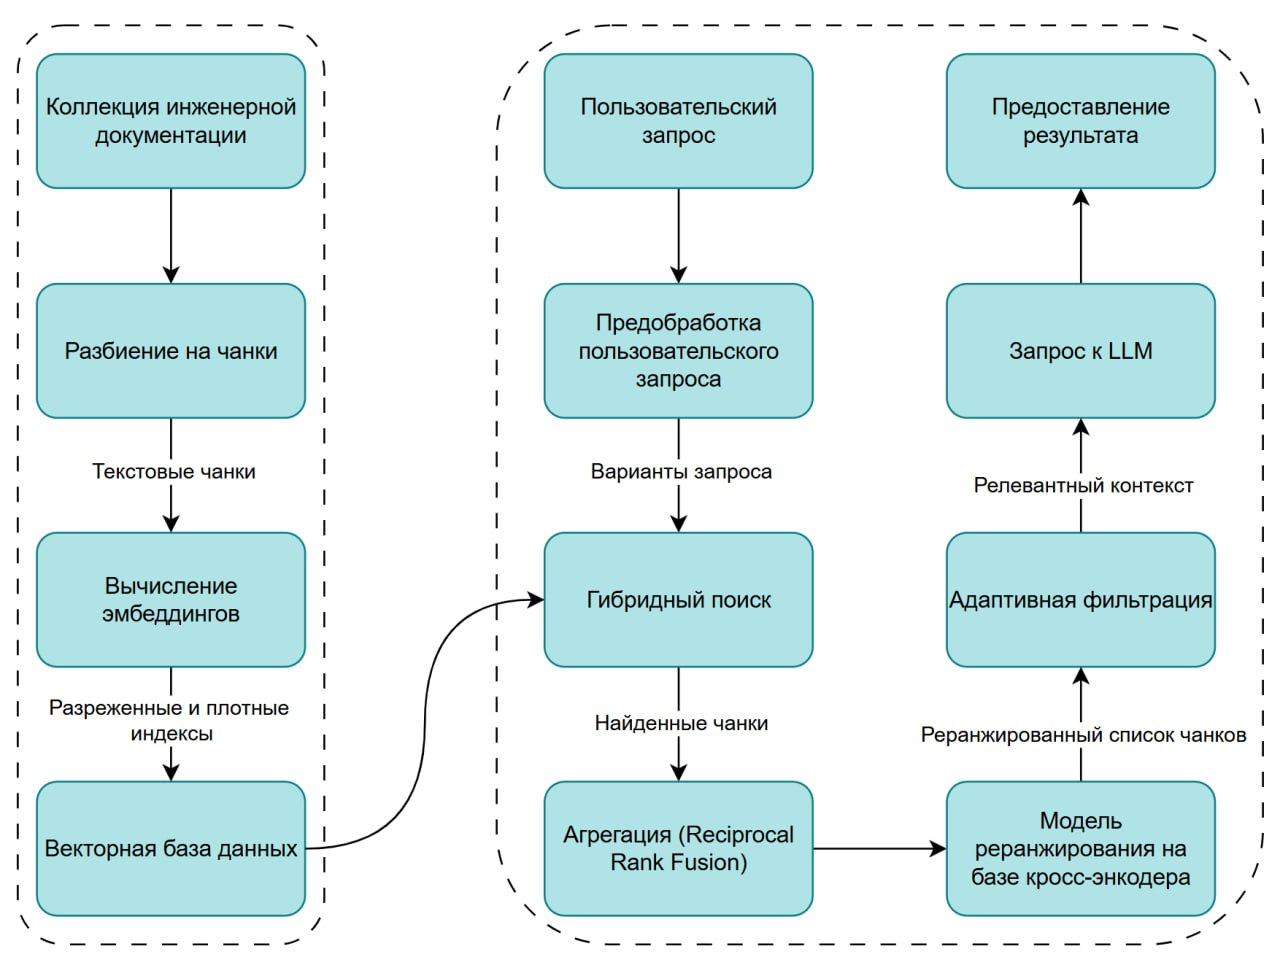
\includegraphics[width=\textwidth, height=0.85\textheight, keepaspectratio]{scheme2.jpeg}
\end{center}
\end{frame}

% --- Слайд 13 ---
\begin{frame}
\frametitle{Условия проведения тестирования}
\Large
Тестирование системы проводилось на базе вопросов пользователей программных продуктов компании ``ИндорСофт'' и обучающей документации на официальном сайте той же компании.
\end{frame}

% --- Слайд 14 ---
\begin{frame}
\frametitle{Тестирование эмбеддеров}
\begin{center}
\resizebox{\textwidth}{!}{%
\begin{tabular}{|l|c|c|c|c|}
    \hline
    \rowcolor{tabgreen} \textbf{Модель} & \textbf{Faithfulness} & \textbf{Context Recall} & \textbf{Context Precision} & \textbf{Answer Accuracy} \\ \hline
    BGE-M3 & 0,76 & 0,63 & 0,30 & 0,60 \\ \hline
    mGTE & 0,73 & 0,63 & 0,29 & 0,59 \\ \hline
    E5+Splade & 0,53 & 0,40 & 0,14 & 0,36 \\ \hline
    E5+BM25 & 0,74 & 0,63 & 0,34 & 0,59 \\ \hline
    RuBGE & 0,61 & 0,52 & 0,24 & 0,57 \\ \hline
    Fasttext (FB) + BM25 & 0,54 & 0,46 & 0,20 & 0,52 \\ \hline
    Fasttext (RV) + BM25 & 0,59 & 0,42 & 0,21 & 0,51 \\ \hline
\end{tabular}%
}
\end{center}
\end{frame}

% --- Слайд 15 ---
\begin{frame}
\frametitle{Сравнение языковых моделей в роли генератора}
\begin{center}
\resizebox{0.65\textwidth}{!}{%
\begin{tabular}{|l|c|}
    \hline
    \rowcolor{tabgreen} \textbf{Модель} & \textbf{Faithfulness} \\ \hline
    Qwen-4b-instruct & 0,59 \\ \hline
    gpt-oss-20b & 0,76 \\ \hline
    Deepseek v3.2 & 0,87 \\ \hline
\end{tabular}%
}
\end{center}
\end{frame}

% --- Слайд 16 ---
\begin{frame}
\frametitle{Reranking}
\begin{center}
\resizebox{\textwidth}{!}{%
\begin{tabular}{|l|c|c|c|c|}
    \hline
    \rowcolor{tabgreen} \textbf{Модель} & \textbf{Faithfulness} & \textbf{Context Recall} & \textbf{Context Precision} & \textbf{Answer accuracy} \\ \hline
    BGE-M3 & 0,76 & 0,63 & 0,30 & 0,60 \\ \hline
    BGE-M3 + Reranker & 0,76 & 0,69 & 0,43 & 0,75 \\ \hline
\end{tabular}%
}
\end{center}
\end{frame}

% --- Слайд 17 ---
\begin{frame}
\frametitle{Итоговая оценка оптимизированной архитектуры}
\begin{center}
\resizebox{\textwidth}{!}{%
\begin{tabular}{|p{6.5cm}|c|c|c|c|}
    \hline
    \rowcolor{tabgreen} \textbf{Конфигурация} & \textbf{Faithfulness} & \textbf{Context Recall} & \textbf{Context Precision} & \textbf{Answer Accuracy} \\ \hline
    Qwen-4b-instruct + BGE-M3 & 0,59 & 0,61 & 0,31 & 0,58 \\ \hline
    gpt-oss-20b + BGE-M3 & 0,76 & 0,63 & 0,30 & 0,60 \\ \hline
    gpt-oss-20b + BGE-M3 + Reranker & 0,76 & 0,69 & 0,46 & 0,75 \\ \hline
    gpt-oss-20b + BGE-M3 + Reranker + Rewriter & 0,77 & 0,76 & 0,52 & 0,77 \\ \hline
    Deepseek v3.2 + BGE-M3 + Reranker + Rewriter & 0,87 & 0,75 & 0,54 & 0,75 \\ \hline
\end{tabular}%
}
\end{center}
\end{frame}

% --- Слайд 18 ---
\begin{frame}
\frametitle{Результаты}
\small
\begin{enumerate}
    \item Проведен теоретический анализ существующих поколений архитектур RAG.
    \item Адаптирована и локализована методика автоматизированной оценки RAGAS.
    \item Разработана стратегия специализированной предобработки данных, включающая иерархическое разделение текста.
    \item Реализован модуль семантической оптимизации запросов.
    \item Реализован механизм гибридного поиска.
    \item Проведен сравнительный анализ эффективности различных LLM.
    \item Проведено сравнительное тестирование современных моделей векторных представлений.
    \item Интегрированы механизмы заключительной обработки.
\end{enumerate}
\end{frame}

% --- Слайд 19 ---
\begin{frame}
\vspace{2cm}
\centering
\Huge \textbf{Спасибо за внимание!}
\end{frame}

\end{document}